\documentclass[tikz,border=4pt,12pt]{standalone}
\usepackage{graphicx}
\usepackage{xcolor}
\usetikzlibrary{positioning,arrows.meta}
\begin{document}
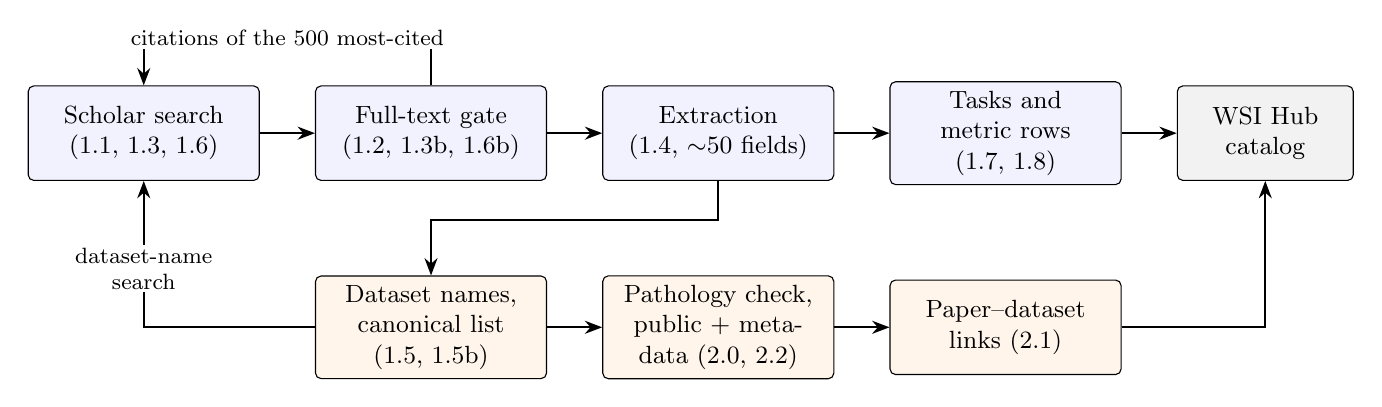
\begin{tikzpicture}[
  node distance=12mm and 7mm,
  box/.style={draw, rounded corners=2pt, align=center, font=\small, minimum height=12mm, text width=27mm, fill=blue!5},
  dbox/.style={box, fill=orange!8},
  lab/.style={font=\footnotesize, fill=white, inner sep=1pt},
  arr/.style={-{Stealth[length=2.2mm]}, thick}]
\node[box] (s) {Scholar search\\(1.1, 1.3, 1.6)};
\node[box, right=of s] (g) {Full-text gate\\(1.2, 1.3b, 1.6b)};
\node[box, right=of g] (e) {Extraction\\(1.4, ${\sim}$50 fields)};
\node[box, right=of e] (m) {Tasks and\\metric rows (1.7, 1.8)};
\node[dbox, below=of g] (d) {Dataset names,\\canonical list (1.5, 1.5b)};
\node[dbox, right=of d] (v) {Pathology check,\\public + metadata (2.0, 2.2)};
\node[dbox, right=of v] (l) {Paper--dataset\\links (2.1)};
\node[box, right=of m, fill=gray!10, text width=20mm] (h) {WSI Hub\\catalog};
\draw[arr] (s) -- (g); \draw[arr] (g) -- (e); \draw[arr] (e) -- (m); \draw[arr] (m) -- (h);
\draw[arr] (e.south) -- ++(0,-5mm) -| (d.north);
\draw[arr] (d) -- (v); \draw[arr] (v) -- (l); \draw[arr] (l) -| (h.south);
\draw[arr] (g.north) -- ++(0,6mm) -| node[lab, pos=0.25] {citations of the 500 most-cited} (s.north);
\draw[arr] (d.west) -| node[lab, pos=0.7, align=center] {dataset-name\\search} (s.south);
\end{tikzpicture}
\end{document}
